\chapter{Description des données}

Les données proviennent du parc photo-voltaïque de Blond, géré par Solaire Direct une filiale d'Engie.
Elles sont groupées en trois catégories:
\begin{itemize}
\item Données électriques au pas de temps minute représentant la production électrique brute et modélisée par Engie
\item Données météo comme l'irradiance, la température, la pluviométrie, la hygrométrie et la vitesse du vent
\item Données de maintenance des équipements
\end{itemize}

Ces données alimentent une base de donnée SQL Server nommée « Agrégation / Reporting ».
Engie procède à l'extraction de l'ensemble des données depuis la base SQL et met à disposition de l'équipe Télécom Paristech un lot de fichiers plats au format csv.

La liste des fichiers plats csv reçus est la suivante:
\begin{itemize}
\item PV.csv
\item INVERTER.csv
\item ITS.csv
\item PLANT.csv
\item PCI.csv
\item architecture.xlsx
\item WEATHER\_STATION\_DATA\_SETS.csv
\item EVENT.csv
\end{itemize}

L'ensemble des fichiers contient des données brutes sur 18 mois, excepté le fichier PV.csv qui contient des données déjà formatées et nettoyées sur 5 mois.
Pour le moment, ce sont les données provenant de ce fichier qui sont utilisées.


\section{Données formatées/nettoyées}

Ces données formatées/nettoyées sont fournies au niveau du fichier « PV.csv ». Elles sont échantillonnées dans le temps avec un pas de 10 minutes et contiennent des informations sur l'irradiance, sur la puissance produite et agrégée au niveau de l'onduleur(inverter en anglais).
Nous avons 8 onduleurs différents.

En plus de la puissance produite et de l'irradiance nous avons deux colonnes supplémentaires concernant la puissance prédite par deux modèles différents créés par Engie.
La puissance prédite dans la colonne « Pred\_self » provient d'un modèle qui prend en compte les données électriques ainsi que les divers données météo. 
La puissance prédite dans la colonne « Pred\_neighbour » provient d'un modèle qui prend en compte la puissance produite par les onduleurs voisins. 

\begin{figure}[!ht]
\begin{center} 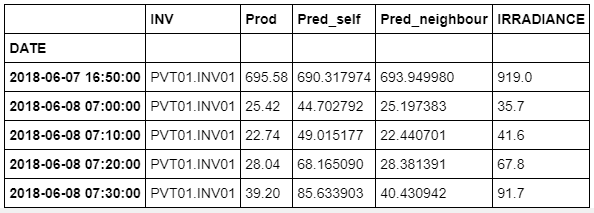
\includegraphics[scale=0.8]{rapport/images/Ch51_PV_head.png} \end{center}
\caption{Extrait du fichier PV.csv}
\end{figure}

\newpage
\section{Données brutes}
\subsection{Les données électriques}

Les données électriques sont collectées au niveau de chaque onduleur, mais elles sont également agrégées à plusieurs niveaux jusqu'à la ferme solaire entière. 

La structure de la ferme solaire est constituée de différents équipements, avec les feuilles représentant les onduleurs (INV), ensuite les transformateurs (ITS), les antennes (FEEDER) et l'entité qui représente la ferme solaire (PLANT).

\begin{figure}[!ht]
\begin{center} 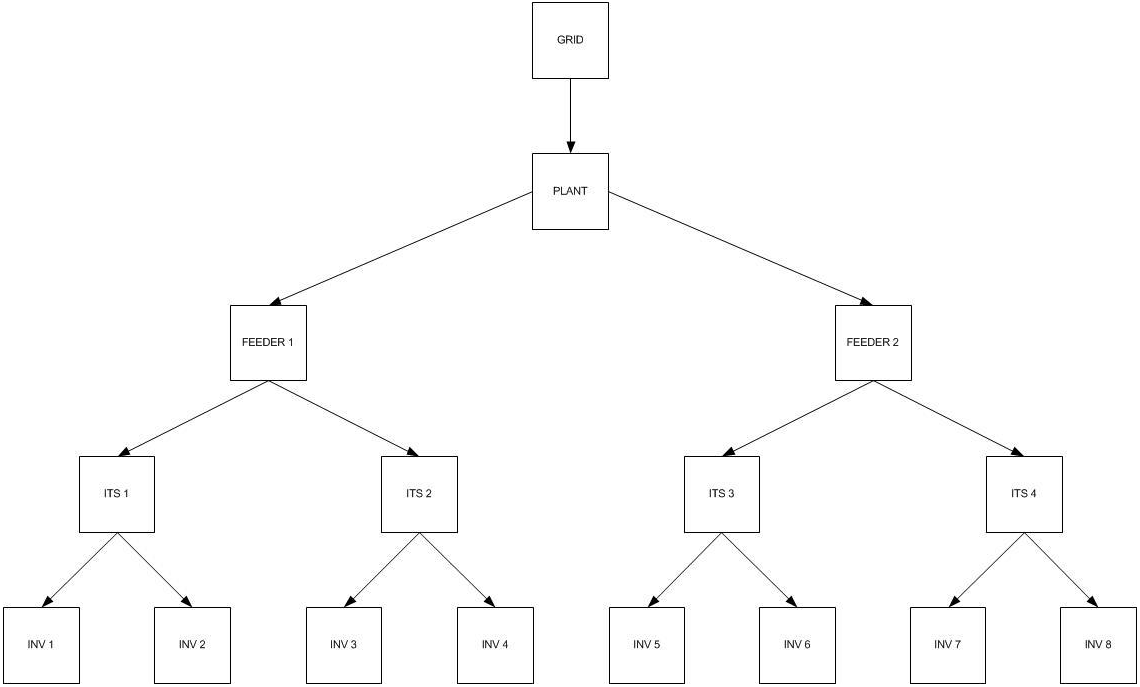
\includegraphics[scale=0.5]{rapport/images/Ch51_equipements_parc.png} \end{center}
\caption{Équipements de la ferme solaire}
\end{figure}

\newpage

Le fichier « INVERTER.csv » contient les mesures effectuées toutes les minutes du voltage, de l'intensité du courant, de la résistance d’isolement, de la température interne, de la puissance active, de la puissance réactive ainsi que de la puissance active produite depuis la mise en service.

\begin{table}[htb]
\resizebox{15cm}{!}{
\begin{center}
   \begin{tabular}{ || l | l|| }
     \hline
     \rowcolor{lightgray} \ \  Nom de la colonne & Description \\ \hline
     DATE & La date à laquelle les mesures ont été effectuées \\ \hline
     INVERTER\_ID & L'identifient de l'onduleur \\ \hline
     DC\_VOLTAGE & U DC, V \\ \hline
     AC\_VOLTAGE\_U12 & U12, V \\ \hline
     AC\_VOLTAGE\_U23 & U23, V \\ \hline
     AC\_VOLTAGE\_U31 & U31, V \\ \hline
     DC\_CURRENT & I DC, A \\ \hline
     AC\_CURRENT\_I12 & I12, A \\ \hline
     AC\_CURRENT\_I23 & I23, A \\ \hline
     AC\_CURRENT\_I31 & I31, A \\ \hline
     INSULATION\_RESISTANCE  & Résistance d’isolement \\ \hline
     INTERNAL\_TEMPERATURE\_1 & Température interne 1, \degree C \\ \hline
     INTERNAL\_TEMPERATURE\_2 & Température interne 2, \degree C \\ \hline
     INTERNAL\_TEMPERATURE\_3 & Température interne 3, \degree C \\ \hline
     ACTIVE\_POWER & P, kW \\ \hline
     REACTIVE\_POWER & Q, kVAr \\ \hline
     COMMISSIONING\_ACCUMULATED\_ACTIVE\_ETU & Comptage d'énergie active produite depuis MES, kWh \\ 
     \hline
   \end{tabular}
 \end{center}}
\caption{La structure du fichier INVERTER.csv }
\end{table}

Le fichier « ITS.csv » regroupe des mesures de températures et d'irradiance au niveau des transformateurs qui regroupent deux onduleurs. Ces mesures sont réalisées tous les 10 minutes.

\begin{table}[htb]
\resizebox{15cm}{!}{
\begin{center}
   \begin{tabular}{ || l | l|| }
     \hline
     \rowcolor{lightgray} \ \  Nom de la colonne & Description \\ \hline
     DATE & La date à laquelle les mesures ont été effectuées  \\ \hline
     ITS\_ID  & Identifiant de l’ITS associé  \\ \hline
     GT\_IRRADIANCE &  Irradiance POA, W/{\SI{}{\metre\squared}} \\ \hline
     MODULE\_TEMPERATURE  & Température sous module, \degree C \\ \hline
     SHELTER\_HV\_TEMPERATURE  & Température local HT, \degree C \\ \hline
     SHELTER\_LV\_TEMPERATURE  & Température local BT, \degree C \\
     \hline
   \end{tabular}
 \end{center}}
\caption{La structure du fichier ITS.csv }
\end{table}

\newpage

Le fichier « PLANT.csv » contient les mesures électriques agrégées toutes les minutes au niveau de la ferme solaire entière.

\begin{table}[htb]
\resizebox{15cm}{!}{
\begin{center}
   \begin{tabular}{ || l | l|| }
     \hline
     \rowcolor{lightgray} \ \  Nom de la colonne & Description \\ \hline
     DATE & La date à laquelle les mesures ont été effectuées \\ \hline
     PLANT\_ID & Identifiant du parc \\ \hline
     DAILY\_ACCUMULATED\_GT\_IRRADIANCE & Cumul irradiance POA journalier, Wh/{\SI{}{\metre\squared}} \\ \hline
     REF\_IRRADIANCE & Irradiance de Référence, W/{\SI{}{\metre\squared}} \\ \hline
     ACTIVE\_POWER\_CONSUMED & Puissance active consommée, kW \\ \hline
     REACTIVE\_POWER\_CONSUMED & Puissance réactive consommée, kVAr \\ \hline
     U12\_AUX\_ELEC\_METER & U12, V \\ \hline
     U23\_AUX\_ELEC\_METER & U23, V \\ \hline
     U31\_AUX\_ELEC\_METER & U31, V \\ \hline
     INSTANT\_ACTIVE\_POWER & Puissance active instantanée, kW \\ \hline
     INSTANT\_REACTIVE\_POWER & Puissance réactive instantanée, kVAr \\ \hline
     COMMISSIONING\_ACCUMULATED\_ACTIVE\_EFU & Comptage d'énergie active consommée depuis MES, kWh \\ \hline
     COMMISSIONING\_ACCUMULATED\_ACTIVE\_ETU & Comptage d'énergie active produite depuis MES, kWh \\ \hline
     COMMISSIONING\_ACCUMULATED\_REACTIVE\_EFU & Comptage d’énergie réactive consommée depuis MES, kVArh \\ \hline
     COMMISSIONING\_ACCUMULATED\_REACTIVE\_ETU & Comptage d'énergie réactive produite depuis MES, kVArh \\ \hline
     DAILY\_ACCUMULATED\_ACTIVE\_EFU & Comptage journalier d'énergie active consommée, kWh \\ \hline
     DAILY\_ACCUMULATED\_ACTIVE\_ETU & Comptage journalier d'énergie active produite, kWh \\ \hline
     DAILY\_ACCUMULATED\_REACTIVE\_EFU & Comptage journalier d’énergie réactive consommée, kVArh \\ \hline	 
     DAILY\_ACCUMULATED\_REACTIVE\_ETU & Comptage journalier d'énergie réactive produite, kVArh \\ \hline	 
     U12\_SD\_ELEC\_METER & U12, V \\ \hline	 
     U23\_SD\_ELEC\_METER & U23, V \\ \hline	 
     U31\_SD\_ELEC\_METER & U31, V \\
     \hline
   \end{tabular}
 \end{center}}
\caption{La structure du fichier PLANT.csv }
\end{table}

Le fichier « PCI.csv » fournit la puissance crête installée à plusieurs niveaux d'agrégation à partir des boîtiers de raccordement jusqu'à la ferme solaire entière. Les données contenues dans ce fichier ne sont pas temporelles. 

\begin{table}[htb]
{\fontsize{6}{8} \selectfont 
\resizebox{15cm}{!}{
\begin{center}
   \begin{tabular}{ || l | l|| }
     \hline
     \rowcolor{lightgray} \ \  Nom de la colonne & Description \\ \hline
     P\_ID & Identifiant de la ferme solaire  \\ \hline
     P\_NAME & Nom de la ferme solaire  \\ \hline
     P\_PCI & Puissance crête installée de la ferme solaire \\ \hline
     F\_ID & Identifiant de l'antenne \\ \hline
     F\_NAME & Nom de l'antenne \\ \hline
     F\_PCI & Puissance crête installée de l'antenne \\ \hline
     ITS\_ID & Identifiant du transformateur \\ \hline
     ITS\_NAME & Nom du transformateur \\ \hline
     ITS\_PCI & Puissance crête installée du transformateur \\ \hline
     INV\_ID & Identifiant de l'onduleur \\ \hline
     INV\_NAME & Nom de l'onduleur \\ \hline
     INV\_PCI & Puissance crête installée de l'onduleur \\ \hline
     AB\_ID & Identifiant du boîtier de raccordement(array box) \\ \hline
     AB\_NAME & Nom du boîtier de raccordement(array box) \\ \hline
     AB\_PCI & Puissance crête installée boîtier de raccordement(array box) \\	 
     \hline
   \end{tabular}
 \end{center}}}
\caption{La structure du fichier PCI.csv }
\end{table}

\newpage

Le fichier « architecture.xlsx » contient la table de correspondance entre les identifiants et les noms des différents composants de la ferme solaire. 

\begin{table}[htb]
\resizebox{15cm}{!}{
\begin{center}
   \begin{tabular}{ || l | l|| }
     \hline
     \rowcolor{lightgray} \ \  Nom de la colonne & Description \\ \hline
     ETL\_ID & Identifiant de l'extracteur ETL \\ \hline
	 ETL\_NAME & Type de l'extracteur (temps réel ou différé) \\ \hline
     PLANT\_ID & Identifiant de la ferme solaire \\ \hline
     PLANT\_NAME & Nom de la ferme solaire \\ \hline
     WEATHER\_STATION\_ID & Identifiant de la station météo \\ \hline
     WEATHER\_STATION\_NAME & Nom de la station météo \\ \hline
     FEEDER\_ID & Identifiant de l'antenne \\ \hline
     FEEDER\_NAME & Nom de l'antenne \\ \hline
     ITS\_ID & Identifiant du transformateur \\ \hline
     ITS\_NAME & Nom du transformateur \\ \hline
	 INVERTER\_ID & Identifiant de l'onduleur \\ \hline
     INVERTER\_NAME & Nom de l'onduleur \\ \hline
     ARRAY\_BOX\_ID & Identifiant du boîtier de raccordement(array box) \\ \hline
     ARRAY\_BOX\_NAME & Nom du boîtier de raccordement(array box) \\
     \hline
   \end{tabular}
 \end{center}}
\caption{La structure du fichier architecture.xlsx }
\end{table}

\subsection{Les données météo}

Les données météo en dehors de la température se retrouvent au niveau du fichier « WEATHER\_STATION\_DATA\_SETS.csv ». Il contient les valeurs de l'irradiance, de la température, de la pluviométrie, de la hygrométrie et de la vitesse du vent. La température et l'irradiance sont collectées tous les minutes, alors que la pluviométrie, la hygrométrie et la vitesse du vent sont enregistrées tous les 10 minutes seulement.

\begin{table}[htb]
\resizebox{15cm}{!}{
\begin{center}
   \begin{tabular}{ || l | l|| }
     \hline
     \rowcolor{lightgray} \ \  Nom de la colonne & Description \\ \hline
     DATE & Horodate associée aux valeurs \\ \hline
	 WEATHER\_STATION\_ID & Identifiant de la station météo associée \\ \hline
     HYGROMETRY & Hygrométrie, \\ \hline
     GH\_IRRADIANCE & Irradiance GHI, W/{\SI{}{\metre\squared}} \\ \hline
     PLUVIOMETRY & Pluviométrie, mm \\ \hline
     GT\_IRRADIANCE & Irradiance GT station météo, W/{\SI{}{\metre\squared}} \\ \hline
     AMBIENT\_TEMPERATURE & Température ambiante extérieure, \degree C \\ \hline
     WIND\_SPEED & Vitesse du vent, m/s \\
     \hline
   \end{tabular}
 \end{center}}
\caption{La structure du fichier WEATHER\_STATION\_DATA\_SETS.csv }
\end{table}

\subsection{Données de maintenance des équipements}

Les données contenues dans le fichier « EVENT.csv » répertorient les différents événements de maintenance des équipements de la ferme solaire, issues du ou des Cahiers Des Incidents déjà existants (conservation de la mémoire des parcs). 
Dans ce fichier nous retrouvons également différentes colonnes contenant le calcul des énergies non distribuées (END) suite à l'événement courant.

\begin{table}[htb]
\resizebox{15cm}{!}{
\begin{center}
   \begin{tabular}{ || l | l|| }
     \hline
     \rowcolor{lightgray} \ \  Nom de la colonne & Description \\ \hline
     ID & Identifiant de l’événement \\ \hline
	 GROUP\_ID & Identifiant du groupe lorsque l’événement fait partie d’un groupe \\ \hline
     NB\_END\_EVENTS\_IN\_GROUP & Nombre d’événements dans un groupe \\ \hline
     STATUS & Etat de l’événement \\ \hline
     START\_DATE & Date de début \\ \hline
     END\_DATE & Date de fin \\ \hline
     TOTAL\_DURATION & Durée de l’événement \\ \hline
     PLANT\_ALIAS & Alias de la ferme solaire \\ \hline
     FEEDER\_ALIAS & Alias de l'antenne \\ \hline
     ITS\_ALIAS & Alias du transformateur \\ \hline
	 INVERTER\_ALIAS & Alias de l'onduleur \\ \hline
     ARRAY\_BOX\_ALIAS & Alias du boîtier de raccordement \\ \hline
     ROOT\_CAUSE & Root cause associée \\ \hline
     ASSIGNMENT\_REPORTING & Description de l’affectation de l’événement \\ \hline
     DESCRIPTION & Description de l’événement \\ \hline
     END\_TOTAL & La valeur de l’END calculée, kWh \\ \hline
     END\_SD & La part Solaire Direct de l’END calculée, kWh \\ \hline
     END\_NOT\_SD & La part non Solaire Direct de l’END calculée, kWh \\ \hline
     FULL\_NAME & Non renseigné \\ \hline
     DELETED\_AT & Date de suppression de l’événement \\ \hline	 
     WITH\_MISSING\_DATA & Booléen indiquant qu’il y a au moins une donnée manquante pour effectuer le calcul de l’END \\	 
     \hline
   \end{tabular}
 \end{center}}
\caption{La structure du fichier EVENT.csv }
\end{table}

La cause ou le type de l'événement est situé au niveau du champ « ROOT\_CAUSE » et peu prendre une des valeurs suivantes :

\begin{itemize}
\item FEEDER\_CIRCUIT\_BREAKER\_OPENED
\item FEEDER\_LOCAL\_CONTROL\_MODE
\item INVERTER ACTIVE POWER NULL
\item INVERTER\_COM\_FAIL
\item INVERTER\_STAND\_BY\_STATUS
\item INVERTER\_STOP\_STATUS
\item ITS\_CIRCUIT\_BREAKER\_OPENED
\item ITS\_LOCAL\_CONTROL\_MODE
\item PLANT ACTIVE POWER LIMITATION VALUE
\item PLANT\_EMERGENCY\_STOP\_REQUEST
\item PLANT\_GRID\_DISCONNECT\_REQUEST
\item PLANT\_GRID\_WAIT\_FOR\_AUTHOR
\item PLANT\_GTE\_TRIP
\item PLANT INSTANT ACTIVE POWER NULL
\item PLANT\_MAIN\_CIRCUIT\_BREAKER\_OPENED
\end{itemize}

Note : à cette date nous attendons encore de confirmer la signification exact de chaque type d'événement afin d'inclure ces informations dans nos jeux de données.